% 2006 湖南理科候选卷 Q9；正四面体过顶点棱与对棱中点的球面截面示意，不按比例标尺寸。
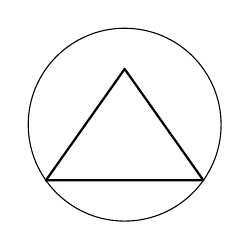
\begin{tikzpicture}[line cap=round,line join=round]
  \coordinate (O) at (0,0);
  \coordinate (L) at (-1,-0.7071);
  \coordinate (R) at (1,-0.7071);
  \coordinate (T) at (0,0.7071);

  % Sphere-section circle and its triangular intersection with the tetrahedron.
  \draw[thin] (O) circle[radius=1.2247];
  \draw[thick] (L)--(R)--(T)--cycle;
\end{tikzpicture}
